\subsection{Transacções e Controlo de Concorrência}

Para o controlo de concorrência é usada a abordagem \textit{TimeStamp Ordering}[1]. Antes de iniciarem, todos os pedidos que vão constituir transações já possuem um \textit{timestamp} atribuído previamente pelo \textit{master}. Isto permite impor a ordem de acesso aos dados e consequentemente resolver os conflitos mais cedo. Deste modo, caso uma transacção queira escrever num objecto que já foi lido por uma transacção com \textit{timestamp} superior ao seu, detecta-se logo que isto não é válido, porque não mantinha a coerência dos dados. Assim que esta anomalia é detectada, o coordenador é avisado pelo servidor e posteriormente é  feito \textit{abort} da transacção em questão. Deste modo, reduz-se a quantidade de trabalho desperdiçado, devido à detecção precoce de anomalias. O mesmo se aplica caso uma transacção queira escrever ou ler num objecto que foi escrito por uma transacção com \textit{timestamp} superior. Tome-se por excepção o caso em que uma transacção tenta escrever num objecto que já foi escrito por uma transacção com \textit{timestamp} superior, não tendo este objecto ainda ter sido lido por outra transacção. Neste caso a escrita atrasada pode ser ignorada ao invés de ser feito \textit{abort}, visto que ia ser sobreposta. Isto pode poupar recursos na medida em que se diminui o número de transacções que reiniciam.

Outra vantagem desta abordagem é que não existem \textit{deadlocks}. Além disto, quando uma transacção chega ao fim sabemos que pode fazer \textit{commit}, pois caso existisse alguma anomalia já tinha sido detectada anteriormente. Caso exista no \textit{log} versões em vias de \textit{commit} e que a transacção actual precisa de ler, a abordagem escolhida é esperar pelo \textit{commit} da outra transacção para prosseguir. Apesar da espera isto será transparente para o cliente.

Quando o cliente faz o pedido ao \textit{master} (com o método \textit{TxBegin()}) e este lhe responde com o \textit{timestamp}, o cliente  dá início à transacção, enviando o pedido, juntamente com o \textit{timestamp} para o servidor responsável por essa nova transacção. 

\begin{description}
\item[Criação de um Objecto:] Após o coordenador receber a transacção relativa ao pedido do cliente, utiliza a fórmula referida anteriormente (baseada no resto da divisão inteira) para saber em que servidor irá ser alojado aquele objecto. Em consequência, o servidor sobre o qual recaiu a responsabilidade de alojar o novo objecto é notificado sobre a criação do mesmo. Esse servidor, cria a sua versão de tentativa transaccional e caso tudo corra bem, o servidor notifica o coordenador que foi tudo feito com sucesso e que pode prosseguir com o \textit{commit}. Seguidamente o coordenador com o \textit{TxCommit()} permite que os dados sejam guardados de forma persistente (com a referência do \textit{timestamp} associado à transacção que efectuou essa criação), avisando posteriormente o cliente que a operação foi efectuada com sucesso. Caso o objecto já exista, é retorna \textit{null} e o servidor avisa o coordenador da situação, sendo que este último utiliza o \textit{TxAbort()}, avisando posteriormente o cliente que a operação não foi efectuada com sucesso.

\item[Acesso a um Objecto:] O processo de leitura ou escrita é semelhante ao da criação do objecto, na medida em que também é usada a mesma fórmula para encontrar a localização do objecto. A diferença reside no facto em que os acessos de leitura ou escrita seguem a metodologia do \textit{TimeStamp Ordering}[1] referida anteriormente, comparando sempre os \textit{timestamps} da transacção actual com o \textit{timestamp} de referência (\textit{timestamp} da última transacção que manipulou o objecto com sucesso). Durante o processo, caso existam anomalias é lançada a excepção \textit{TxException} e o servidor avisa o coordenador da situação, onde este aborta a operação com o mesmo método referido anteriormente.
\end{description}

\begin{figure}
\centering
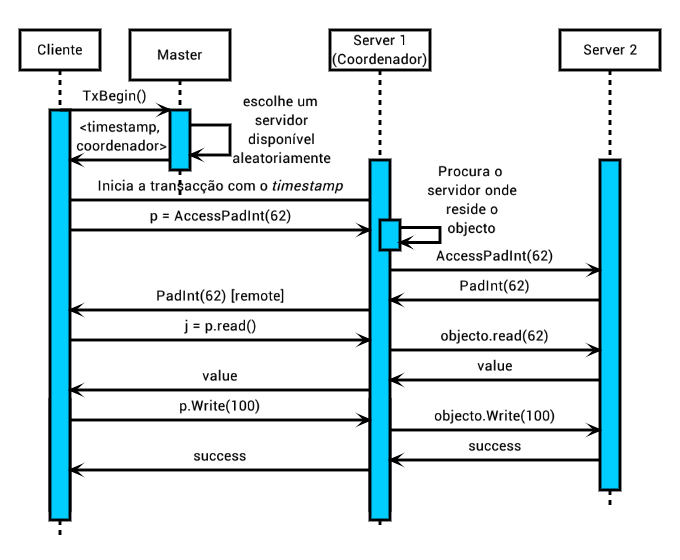
\includegraphics[width=0.4\textwidth]{transaccao.png}
\caption{\label{fig:transaccao}Diagrama transaccional.}
\end{figure}